\documentclass{article} % For LaTeX2e

\usepackage{nips15submit_e,times}
\usepackage{hyperref}
\usepackage{url}
\usepackage{amsmath}
\usepackage{amsfonts}
% \usepackage{graphicx}
\usepackage{array,multirow,graphicx}
\usepackage{subcaption}
% \documentstyle[nips14submit_09,times,art10]{article} % For LaTeX 2.09

\usepackage{booktabs}

\title{Text2Scene Generation \\ Discriminator \& Brutal-force search}


\author{
%David S.~Hippocampus\thanks{ Use footnote for providing further information
%about author (webpage, alternative address)---\emph{not} for acknowledging
%funding agencies.} \\
%Department of Computer Science\\
%Cranberry-Lemon University\\
%Pittsburgh, PA 15213 \\
%\texttt{hippo@cs.cranberry-lemon.edu} \\
%\And
%Coauthor \\
%Affiliation \\
%Address \\
%\texttt{email} \\
%\AND
%Coauthor \\
%Affiliation \\
%Address \\
%\texttt{email} \\
%\And
%Coauthor \\
%Affiliation \\
%Address \\
%\texttt{email} \\
%\And
%Coauthor \\
%Affiliation \\
%Address \\
%\texttt{email} \\
%(if needed)\\
}


% The \author macro works with any number of authors. There are two commands
% used to separate the names and addresses of multiple authors: \And and \AND.
%
% Using \And between authors leaves it to \LaTeX{} to determine where to break
% the lines. Using \AND forces a linebreak at that point. So, if \LaTeX{}
% puts 3 of 4 authors names on the first line, and the last on the second
% line, try using \AND instead of \And before the third author name.

\newcommand{\fix}{\marginpar{FIX}}
\newcommand{\new}{\marginpar{NEW}}

%\nipsfinalcopy % Uncomment for camera-ready version

\begin{document}


\maketitle

\begin{abstract}
\end{abstract}

\section{Task}
Generate a consistent picture given a query text, using learned discriminators as score functions

\section{Dataset}
The dataset contains clip art pictures and corresponding textual descriptions. A picture is composed of several layers, while a layer can be either one among the four basic types, including background, character, surrounding and decoration. A character or surrounding layer can be further classified into several categories. Each category is attached with exclusive identification code for the convenience of encoding. The detailed category table is shown in Table. \ref{tab: cat-surrounding} and \ref{tab: cat-character}.

\begin{table}[!h]
	\caption{Nested categories that a surrounding layer can be divided into.}
	\centering
	\begin{tabular}{cccc|cc|ccc|cc}
		\toprule
		 \multicolumn{6}{c|}{room} & \multicolumn{5}{c}{landscape} \\
		 \midrule
		  \multicolumn{4}{c|}{object} &  \multicolumn{2}{c|}{abstraction} &  \multicolumn{3}{c|}{city} &  \multicolumn{2}{c}{nature} \\
		 \midrule
		 furniture & appliance & wall & sundries & chart & art & street & building & vehicle & park & wild \\
		 \bottomrule
	\end{tabular}
	\label{tab: cat-surrounding}
\end{table}

\begin{table}[htbp]
	\caption{Nested categories that a character layer can be divided into.}
	\centering
	\resizebox{\columnwidth}{!}{\begin{tabular}{cccccc|ccc|cccc}
	\toprule
	 \multicolumn{6}{c|}{interaction} & \multicolumn{7}{c}{person} \\
	 \midrule
	 occupation & abstraction & emotion & sociable & travel & enjoyment & \multicolumn{3}{c|}{stand} & sit & sport & show & gesture \\
	 \midrule
	& & & & & &  lean & back & front & & & & \\
	\bottomrule
	\end{tabular}}
	\label{tab: cat-character}
\end{table}

For simplicity we will not consider the positions of objects, and the layout of a picture will only touch the layer level. Thus the dimensions of the layout are restricted to the specific categories of the layers, as well as the order of overlapping between layers. In addition, several rules need to be followed when composing a picture. Specifically, the background layer should lie below all other layers while the decoration layer should be on top of all other layers. Either a character layer or a surrounding layer should be contained in a picture, if not both. 

There exists prominent biases in the dataset. For instance, the decoration layer rarely appears in the pictures. Occurrences of the categories are also strongly biased. Though at the same level, ``chart'' appears 19 times in all images, while ``appliance'' or ``vehicle'' only appears once. For character categories, ``stand'' appears 17 times, while ``emotion'' only appears once. As a reference, Fig. \ref{fig: picture-occurrence} shows the occurrences of category keywords across all pictures. The imbalanced distribution of categories will strongly impair the performance of the model. Other biases include that, in almost all cases, the character layer is in front of the surrounding layer. To avoid it becoming too easy to discriminate real and fake pictures, here let us remove this dimension in the composition of the picture. The character layer is now always in front of the surrounding layer. The occlusion ambiguity is thus resolved and our task basically turns into an image retrieval problem. Given a description, we are trying to retrieve the most relevant character and surrounding, and at the same time the character and surrounding should be consistent with each other. Note that to retrieve a background or a decoration is trivial. Since the backgrounds and decorations do not have finer tags, the retrieval is entirely random.

As a reference, there are in total 668 possible combinations of layers in consideration of different categories. The number of combinations ever appear in the dataset is near a hundred. Thus there are quite a lot combinations that may not be reasonable. 

At this moment 92 pairs of pictures and descriptions are available. The above investigation and the following training and evaluation are all based on these pairs.

%\begin{table}
%	\caption{The reference sheet for layer classification.}
%	\centering
%	\begin{tabular}{ccccccccccccc}
%		
%	\end{tabular}
%\end{table}

\section{Feature engineering}
We decide to build the discriminator with either a simple logistic regression or boosting model to . Thus feature engineering is of great importance in the pipeline. Basically we have to deal with three parts of features in this problem, namely those encoding the textual description, those encoding the picture layout, and the additional ones that jointly encode the relations between the description and the picture.

To deal with the text, we first introduce a tokenizer that transform a sentence into a series of keywords. Specifically, the sentence will be processed into tokens by the \emph{nltk} standard tokenizer, which are then fed into the \emph{nltk} standard POS tagger to identify their associated POS tags. Punctuations and stop words will be removed afterwards. A lemmatizer introduced by WordNet is used to lemmatize the tokens based on their POS tags. And the lemmas are further transformed into WordNet synsets, in aid of the calculations of similarities. Word sense disambiguation will not be mentioned here. Obtained synsets now serve as the keywords in our vocabulary. Unseen tokens will be discarded directly, which is obviously not reasonable and will be fixed later. Once we manage to represent a sentence using keywords included in the vocabulary, a simple Tf-idf vectorizer can be introduced to encode it. Both unigrams and bigrams will be used. The idfs of all keywords in the vocabulary will be scaled linearly such that they range from 0 to 1. As a reference, there will be in total 298 keywords in the vocabulary, including bigrams. The occurrences of keywords are biased prominently. In Fig. \ref{fig: text-occurrence} we list the keywords that occurs more than once. In fact, there are only 39 such keywords in the entire description corpus. 

\begin{figure}[htbp]
  	\centering
	\begin{subfigure}{.42\linewidth}
	\centering
	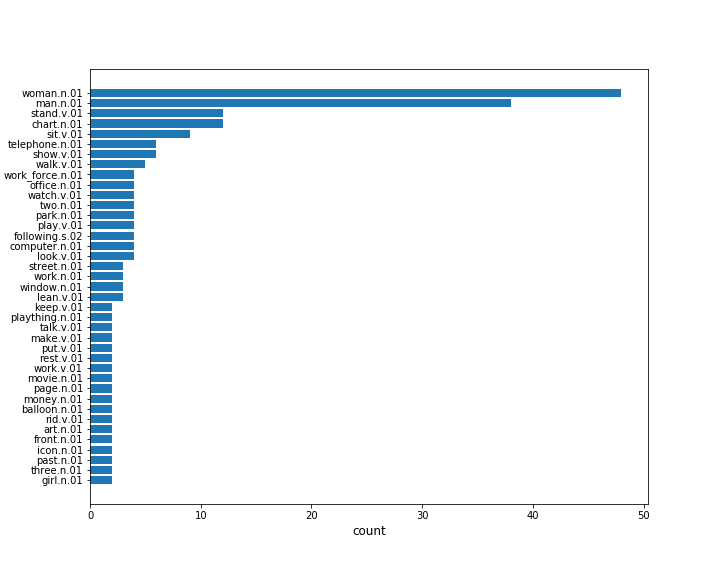
\includegraphics[width=\linewidth]{../Text2Scene/results/text-occurrence}
	\caption{Keywords that occurs more than once in the description corpus}
	\label{fig: text-occurrence}
	\end{subfigure}
	\begin{subfigure}{.57\linewidth}
	\centering
	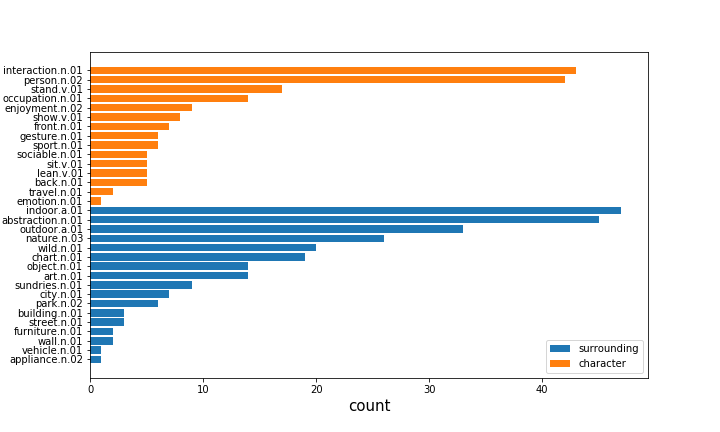
\includegraphics[width=\linewidth]{../Text2Scene/results/picture-occurrence}
	\caption{Occurrences of category keywords across all pictures}
	\label{fig: picture-occurrence}
	\end{subfigure}
	\caption{Histograms of keyword occurrences}
\end{figure}

Next we encode the pictures, or as a matter of fact, only the nested categories a picture belongs to, since we will not touch pixel-wise information, nor any position or attribute information. As mentioned before, there's no finer category to differ the backgrounds or the decorations. Therefore these two layers can be simply encoded to binaries, telling if the layer exists in the picture or not. The character and surrounding layer can be encoded similarly, with two binaries telling if they exists, and two additional binary vectors where each entry indicates whether this specific category gets mentioned or not. There will be a binary vector of length 16 to encode the categorical tags of a character layer, and a vector of length 17 to encode the tags of a surrounding layer. There will also be a feature telling how many layers there are in the picture. Finally, to facilitate the evaluation of the reality of a picture, similarities between each category name associated with character and that associated with surrounding will be counted as features. Here we will use the WordNet \emph{lch} similarity, and the category names will be transformed into most relevant synsets manually. Those similarities will be z-scored such that they have zero mean and unit standard deviation. Consequently, there will be in total 310 features to encode a picture.

Now let us consider the encoding in a different view. Since the pictures only differ from each other in the layer names, as well as the category names each layer associated with, we can actually treat these tags in whole as the image caption. Each picture is then simply a bag of words. And our task becomes to find the most relevant keywords given a description, subject to some constraints that describe the nesting relations. Following this point, we can introduce the tf-idf vectorizer here as well, to suppress the contributions of some most frequent categories. Scaled Idfs can take place of the binary vectors that indicate the occurrence of the layers and categories. They can also reweight the pairwise similarities as mentioned before. The effect of this trick will be discussed later.

In the end, we need to jointly encode the pictures and the textual descriptions such that the consistency between them can be interpreted. We can simply encode this information by constructing a binary table with the row containing all the keywords from the text, and the column containing all the keywords from the picture categories. Each entry then indicates whether a textual keyword and a picture keyword cooccur in a picture-description pair. Similar as before, we can also introduce the \emph{lch} similarity between keywords. As shown in Fig. \ref{fig: cross-simi}, these similarities should be z-scored, otherwise dissimilar keyword pairs will take little effects in inferring the discrepancy between pictures and descriptions. Note that here we will not count the bigrams in the vocabulary. Moreover, \emph{idf} reweighting can be introduced here as well. Idfs of both textual keywords or categorical keywords can be multiplied with pairwise similarities to suppress highly frequent keywords.

\begin{figure}[htbp]
	\centering
	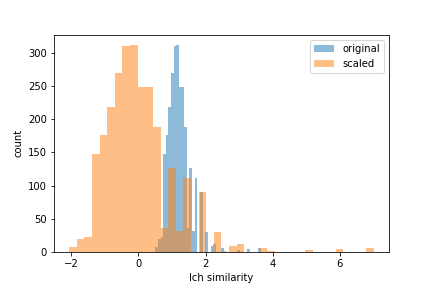
\includegraphics[width=0.5\textwidth]{../Text2Scene/results/cross-simi}
	\caption{The histogram of similarities between text keywords and picture keywords.}
	\label{fig: cross-simi}
\end{figure}

\section{Model and evaluation}
In order to fulfill the text to picture generation task, our idea is to train two discriminators, one to tell consistent description-picture pairs from inconsistent ones, and the other one to tell if a picture is fake or not. These two discriminators can be properly combined into a score function. Then given a piece of query text, we only have to find the one that is scored the highest among all the possible patterns that represent a picture.

\subsection{Consistency discriminator}
To train a consistency discriminator, we need to build a dataset containing both consistent and inconsistent picture-description pairs. A consistent description is simply the one manually generated to describe a picture, while an inconsistent description can be picked from all the descriptions in the corpus randomly, as long as it is different from the original one. Similarly, given a description, we can also retrieve an inconsistent picture from all the pictures we have. Here we do not consider the document-wise similarities between descriptions, nor the picture-wise similarities. Thus we may accidentally retrieve a description very similar to the original one, and to simply label this description as inconsistent may not be appropriate, or at least it may not be as inconsistent as other pairs. A more promising method is to sort all other descriptions with respect to their similarities with the original one. During training, highly dissimilar descriptions are first picked to form inconsistent (negative) pairs, then the less dissimilar ones. This is often known as curriculum learning. 

Specifically, to build the dataset, when given a positive example, namely the true picture-description pairs, we can generate two negative examples correspondingly, which are incorporated into a triplet. Each pair is encoded as mentioned above. Textual, pictorial and joint features are concatenated, yielding in total a sparse feature vector of length 10,442. We can shuffle the true pairs before training. But to maintain the triplet structure is crucial to the performance of the discriminator. 

Now given the dataset, we can train a simple binary classification model. Logistic regression will be used here because of its interpretability. We will introduce the L1 regularizer to encourage a sparse representation. A negative example will be given a weight only the tenth of that of a positive one, to force the learner to focus on the true pairs. 

We randomly choose about 90\% examples to train the discriminator, and test on the rest 10\% ones. The overall accuracy is 0.4, while the accuracy of positive examples, or equivalently the recall, is 0.9. The latter one is more important in judging the performance, but we still needs a more robust metric to evaluate the model. We can either try the precision-recall curve, or the receiver operating characteristic. It turns out the precision-recall curve is more preferred, since we are handling an imbalanced dataset. We show both two metrics in Fig. \ref{fig: consistent-metric}. The associated average precision (AP) and the area-under-curve (AUC) are annotated on the top. We also show the maximum F1 score obtained given different thresholds. Due to the insufficient data, the performance of the discriminator varies prominently as the test set varies. In all, the average precision is about 0.5, which is acceptable. We should use K-folds cross-validation to obtain a more robust evaluation, which will be tried later. 

\begin{figure}[htbp]
	\centering
	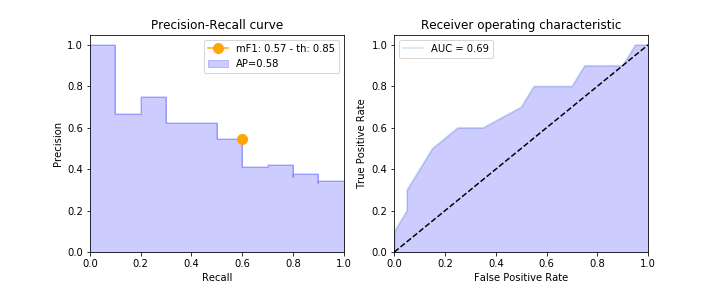
\includegraphics[width=\textwidth]{../Text2Scene/results/ROC_idf*norm-simi2}
	\caption{Precision-recall curve and ROC of the logistic regressor obtained on the test set in discriminating the consistency between a picture and a description}
	\label{fig: consistent-metric}
\end{figure}

\begin{figure}[htbp]
	\begin{subfigure}{0.5\linewidth}
		\centering
		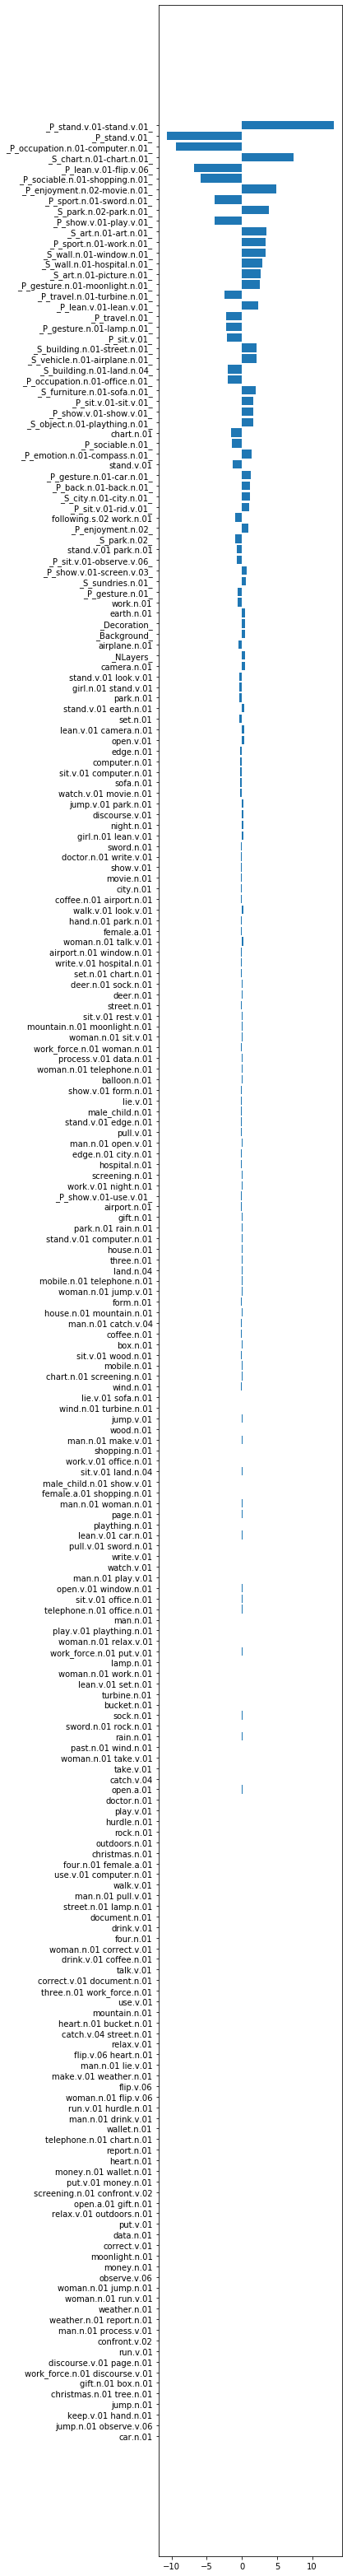
\includegraphics[height=\textheight]{../Text2Scene/results/FEAT_idf*norm-simi2}
		\caption{Most important features in discriminating the consistency between a picture and a description}
		\label{fig: consistent-feat}
	\end{subfigure}
	\begin{subfigure}{0.48\linewidth}
		\centering
		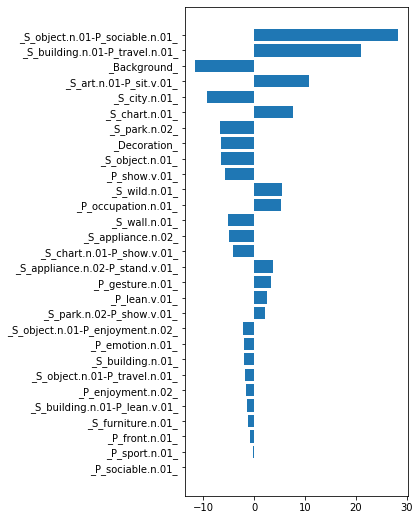
\includegraphics[width=\linewidth]{../Text2Scene/results/realityFEAT_temp}
		\caption{Most important features in discriminating the reasonability of a picture.}
		\label{fig: real-feat}
	\end{subfigure}
\end{figure}

We count the coefficient associated with each feature in the learned logistic regression model as its importance. In Fig. \ref{fig: consistent-feat}, we list the most important features. There are quite a lot interesting things we can discuss in this bar graph. The most contributive features are often those pairs composed of exactly same keywords, for instance, ``stand'' as a category name, paired with ``stand'' as a keyword in the vocabulary.
% ``park'' as a category depicting the surrounding, combined with ``park'' in the text vocabulary, is very helpful to determine if a picture is consistent with the description. This originates from two aspects. One is that their similarity is very high, and the other is that they are not that common across the corpus. The most common keywords, for example, ``chart'' and ``stand'', both occurring frequently as category names in the pictures, and as keywords in the descriptions, are not that prominent in terms of importance. This is mainly thanks to the idf reweighing, which we wish can improve the generality of our model. 
Dissimilar keyword pairs can also contribute to the discrimination. For example, ``show'' and ``play'' as a paired feature helps ruling out the character of showing things when seeing ``play'' in the description. One can notice that the names of finer categories contribute more, obviously because they carry more concrete meaning than the general ones. One can also notice that paired features dominate in the contributive list, which shows the importance of joint encoding. As an additional note, in Chang 2014, a similar discriminator is trained to obtain the most important keyword pairs, which are then used to map keywords in the description to categories in the picture. In this way, we should avoid z-scoring the pairwise similarity features, such that dissimilar pairs will not appear in the list important features, and the model can focus on leveraging the similar keyword pairs. 

Now let us discuss some specific examples that the discriminator made mistakes on. In one example, the description is ``A woman holds a toy.'', while the corresponding picture contains three layers, including a character, a surrounding and a background. The categories associated with the character layer are ``person'' and ``sit'', while the categories associated with the surrounding layer are ``indoor'', ``object'' and ``sundries''. The discriminator mistakenly predicts this pair as inconsistent. Among the non-zero features encoding this particular example, there are quite a few that strongly support the consistency. ``object'' and ``plaything'', the synset name of ``toy'', for instance, are highly similar and at the same time quite distinct among the corpus. However, the learned coefficient corresponding to this feature is 0. In fact, the only two features having non-zero coefficients in this example are the number of layers and the keyword ``woman''. Therefore there's no way for the discriminator to determine the consistency. The problem lie in the shortage of recurrent data.

\subsection{Reasonability discriminator}
Now let us build a dataset to train the reasonability discriminator. The real pictures serve as positive example, while negative examples, namely fake pictures must be generated properly. As mentioned before, there are in total 668 possible combinations of layers that can form a picture. We can simply remove the combinations that ever appeared in the real pictures from all the combinations. The rest can serve as fake pictures. These fake pictures may not be entirely irrational, because first the available pictures are obviously not enough to cover all reasonable combinations, and more importantly, the reasonability of a picture may not be that easy to tell. After all, the reasonability can only depend on the consistencies between the character and surrounding layers, and a few category tags are insufficient to characterize them.

when building the dataset, for each real picture, we randomly choose a fake picture from the fake pool, and jointly feed them to a logistic regressor. Here only the 330 pictorial features are involved.  Similarly we introduce the L1 regularizer, but the classes will share equal weights since the dataset is balanced. Note that here we must ensure that the data used to train this discriminator are same as the training data used above.

In Fig. \ref{fig: real-metric} we show the precision-recall curve and receiver operating characteristic of this discriminator. The model does well, obtaining an average precision of 0.86. In Fig. \ref{fig: real-feat} we list the most important features. Some are reasonable. For example, ``object'' as a type of surrounding is often related to people in ``social'', and ``art'' is often related to people ``sitting''. Nevertheless, there are features contributing to the decision totally due to bias. For instance, in real pictures the decoration layer does not appear very often, and on the contrast, ``wild'' surrounding appears very often. But these should not contribute to the discrimination because the occurrences of particular layers or categories have nothing to do with the reasonability of a picture.

\begin{figure}
	\centering
	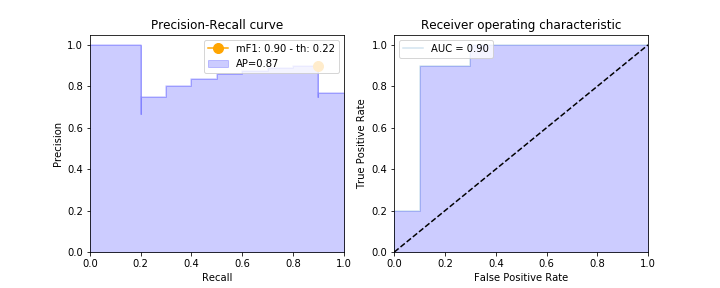
\includegraphics[width=\textwidth]{../Text2Scene/results/realityROC_temp}
	\caption{Precision-recall curve and ROC of the logistic regressor obtained on the test set in discriminating the reasonability of a picture.}
	\label{fig: real-metric}
\end{figure}


\subsection{Generator}
Now that we have the two discriminators, to build a generator is trivial. Given a description, we pair it with all possible pictures (category combinations), then use the consistency discriminator to give the probability that a pair is consistent, and the reasonability discriminator to give the probability that the picture is reasonable. The two probabilities are weighted using a coefficient $\lambda$. The objective is then to find the picture yielding the maximum probability, namely
$$
c^* = \mathop{\arg\max}_{c\in\mathcal{C}} \left[ \lambda P_{cons}(c,t)  + (1-\lambda) P_{reas}(c) \right],
$$
where $c$ represent a possible category combination and $t$ is the query description. This task can be simply performed by a brutal-force search. 

One important thing left is to find a metric to evaluate the generated picture. This is basically same as to quantitate the similarity between pictures. Here we introduce the category-level precision. We first encode the layers and associated categories into binary vectors, which is performed in the picture encoding mentioned above, but leaving the number of layers and pairwise similarities. Then we can measure the similarity of the generated picture with respect to the true picture by the precision and recall of its binary vector compared to the true one. We take the F1 score as a balanced metric, and can be averaged if evaluated on multiple test examples. Our generator achieves a maximum average F1 about $0.58$ on the test set, where $\lambda=0.8$. Again, the choice of the test set strongly affects the performance and the optimal hyper-parameters as well. In Fig. \ref{fig: lamb} we show how the performance of the generator varies with different values of $\lambda$. One can see that the peak locates in between and near $1$, which generally means that the consistency discriminator helps more than the other one, but will be deficient if alone.

\begin{figure}
	\centering
	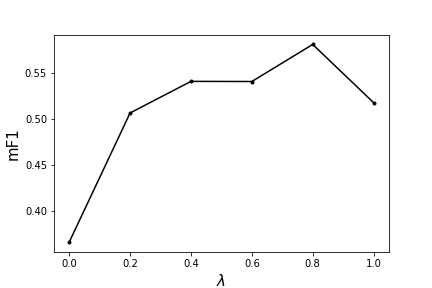
\includegraphics[width=0.5\textwidth]{../Text2Scene/results/generator_lamb-metric}
	\caption{The performance metric of the generator mF1, as the discriminator weight $\lambda$ varies}
	\label{fig: lamb}
\end{figure}

Now let us peer into some specific examples that the generator yields good and poor results. To help with the diagnosis, for each discriminator, we sort the non-zero features learned to non-zero coefficients according to the products between feature values and coefficient values. This is basically a ranking of contribution since we are dealing with a linear model. Between the two discriminators we rank their respective features as well, but according to the same product discounted by the associated weights, which is $\lambda$ for the consistency discriminator and $1-\lambda$ for the reasonability discriminator. This ranking does not reflect the relative contribution realistically, but is rather acceptable under the first-order approximation of the sigmoid function.

Now first, we present an example reported a high F1 score ($>0.82$) and a high confidence\footnote{namely the sum of the weighted probabilities of the two discriminators} ($>0.99$) as well, stating ``A woman is showing two charts.'', with the true picture including a surrounding layer of ``chart'', a character layer of ``gesture'', and an additional decoration layer. This is a rather easy example since there are quite a lot pictures in the dataset related to ``charts showing''. The generator thus grabs a ``chart'' because of the high contribution of the pair  between ``chart'' in the text vocabulary and ``chart'' in the category keywords, a credit to the consistency discriminator. It also grabs a ``show'' because of the feature pair `show-show`'', due to the same reason. Here we have some ambiguity between ``gesture'' and ``show''. But they share a common hypernym, thanks to the nested tagging. In general this is a typical example that the paired similarities between text and pictures are well leveraged.

Here is another typical example that the generator is doing right, but not so confident. The description states ``A woman puts up a lantern.'', while the picture includes a surrounding layer of ``wild'', and a character layer of ``enjoyment''. In fact, the predicted picture is correct entirely. But how the decision is made is not that reasonable. In this case, the mostly contributed feature is actually the number of layers. And no similarity feature appears in the contribution list, probably because the tokens in the description are hard to be connected with the category keywords in terms of similarity. It turns out that the generator retrieves ``wild'' and ``enjoyment'' merely because these two are weighted high by the learners, with the former in the reasonability discriminator and the latter in the consistency discriminator. And that they are weighted is simply due to their high occurrences in the dataset, with ``wild'' the fifth most frequent in the character categories and ``enjoyment'' the fifth most frequent in the surrounding categories. The most frequent keywords like ``stand'' and ``abstraction'' are suppressed because of the idf reweighting. That's how the second class stands out. In all, this example points out the deficiency of our feature engineering. We may try to remove the single tokens in our feature list, and at the same time figure out a better way to jointly encode the similarities between text and picture. This deficiency is also magnified by the sparsity of our dataset. The discriminator may be able to learn the connection between ``lantern'' and ``enjoyment''  spontaneously if multiple examples mention them both. We may replace rare words by their hypernyms to encourage recurrence, but cannot ensure that they all agree on the associated categories.

Now let us look at some examples causing poor performance. There is one description stating ``A woman sat to rest''. The corresponding picture includes a surrounding layer of abstract arts, a character layer of a seated woman, and an additional background layer. The predicted picture is right about the character, which benefits from the contribution from the paired feature ``sit-sit'', but mistakenly presents a wild surrounding, which is due to its high occurrence as the case in the above example. Here, there is no meaningful connection between the description and abstract arts. But an ideal reasonability discriminator should at least capture the consistency between ``sit'' and ``indoor'', thus guiding the generator to retrieve an indoor surrounding. Unfortunately, ``sit'' is a verb while ``indoor'' is an adjective, causing an error when using \emph{lch} similarity. And our model simply returns a zero. This indicates that we may either modify the keywords of the categories, or explore a more compatible algorithm to measure similarity.  

The next example includes a description saying ``A man and a woman are transferring money'', and a picture includes only a character layer of ``sociable'', and an additional background layer. The predicted picture mistakenly includes a redundant surrounding layer. The redundancy of layers is quite common among the predictions. In fact, for the reasonability discriminator, an additional feature with positive contribution, for instance, ``wild'', will always increase the probability, not to mention the positive contribution of the feature associated with the number of layers. Again we should try removing single-token features, or introducing features that can capture the connection between the description and the number of layers. 
%, which we leave aside because there is not a clear pattern between the description and the occurrence of the surrounding.
Another interesting thing in this example is that the predicted picture mistakenly grabs a character layer of ``enjoyment'', but not ``sociable'', again due to the occurrence divergence. But in fact the social activity can be inferred from the existences of both man and woman, which probably requires a feature encoding the similarity between the bigram ``man woman'' and the keyword ``sociable''. We may improve our engineering to incorporate this part into the features.

The final example is a rather difficult one. The description states ``A woman looks in the window'', and the corresponding picture includes a character layer of ``lean'' and a surrounding layer of ``street''. The generator retrieves a ``wall'' for this query because of the high similarity between ``wall'' and ``window'', leading to an ``indoor'' surrounding. And it also retrieves a ``gesture'' because of its contribution in the reasonability discriminator. In this particular case it would be difficult even for human to infer from the sentence it is an indoor or outdoor environment. But it should be fair to infer the person is standing. This surely requires a deeper understanding of semantics.

%\section{Evaluation}
%\subsection{Performance}
%\subsection{Hyperparameters?}
%\subsection{Error analysis}

%\section{Optimization}

\end{document}










